% ##################################################################################################################
\chapter{Germany}
\label{ch:germany}
\hfill \textbf{Author:} Johannes Illenberger

%\editdone{This text has undergone the professional edit. Please no grammatical changes anymore! They are most-probably wrong.}

% ##################################################################################################################
\createfigure%
{}%
{Left: Simulation road network including roads down to the level of major arterials. Right: Spatial distribution of activity facilities colored according to activity type}%
{\label{fig:germany:network}}%
{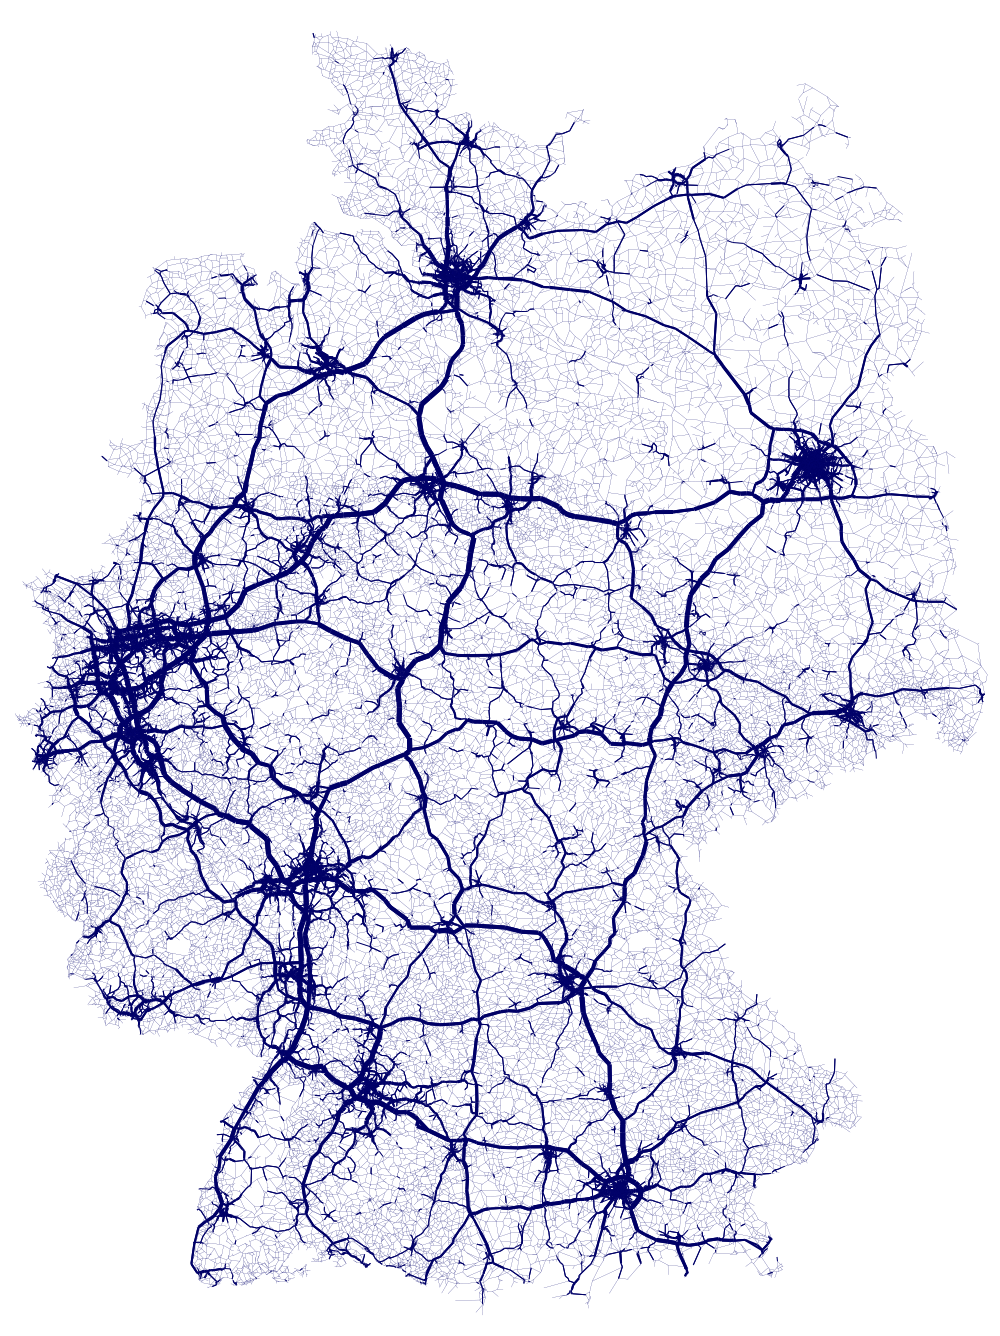
\includegraphics[width=0.45\textwidth, angle=0]{./scenarios/figures/germany-network}\hspace{5mm}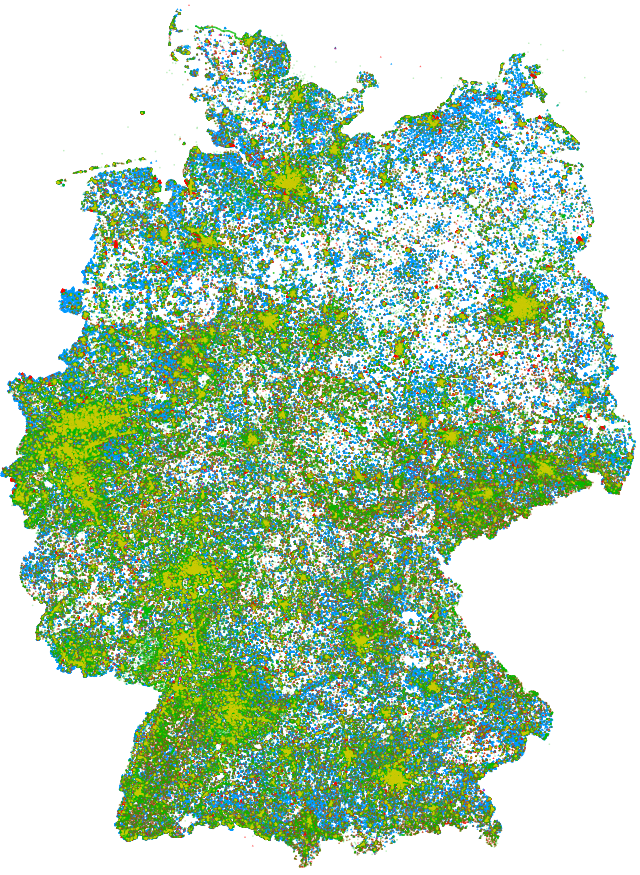
\includegraphics[width=0.45\textwidth, angle=0]{./scenarios/figures/germany-facilities}}%
{}

The Germany scenario is developed from \gls{dbmlag}, a subgroup of \gls{dbag}, the German state-owned railway company, in~2014. To help evaluate \gls{matsim}'s applicability in the strategic planning process, as well as defining its compatibility in the traditional zone-based four-step process, this scenario has been constructed to establish a Germany-wide \gls{od} matrix for private car travel. A solid understanding of the transport market for private car travel (rail's major competitor) is required for the strategic planning process at the \gls{dbmlag}. This scenario intentionally focuses just on road transport since, on one hand, there are already well-established models for rail transport at the \gls{dbmlag} and, on the other hand, this scenario is meant to be the first step towards \gls{matsim}'s application.

Considering this scenario's objective, \gls{matsim} is used here as a tool to build a microscopic representation of the current transport market. Unlike the majority of \gls{matsim} studies, the focus is not to build and calibrate a behavioral model with forecasting power to answer the ``what if'' question. Hence, this study emphasizes reproducing empirical measurements, rather than on modeling plausible causalities and behavioral processes.

The final outcome of this exercise is a \gls{od} matrix with average daily trip volumes. Although a higher temporal resolution is possible and also available from travel data, this dimension will not be considered during calibration and validation of the scenario. The matrix is based on a zonal structure with approx. 10\,K \glspl{taz}, with a granularity comparable to municipalities (\gls{lau} 2) and a higher detail in large cities.

\section{Demand and Supply Data}

The German national travel survey \gls{mid} from 2008 \citep{Follmer2010MiD} builds the foundation for the synthetic population and its travel plans. The survey features approx. 60\,K person records with one-day travel episodes. A travel episode specifies trip sequences with mode, purpose, travel distance and day of reporting. Home locations are known at the level of states and municipality type (urban/rural). From each record, a synthetic person with one travel plan is generated. Initially, activity locations are set to random facilities and each person is cloned multiple times (according to the person's weight), so that in total a population of 4\,M persons results.

The road network is extracted from \gls{osm}. The geographical resolution of the \gls{od} matrix allows omission of minor roads (everything below ``tertiary'' in \gls{osm} terminology)and the network is further simplified so that connected nodes with a distance less than 50\,meter are merged to one node. The resulting network consists of 126\,K nodes and 360\,K links (Figure~\ref{fig:germany:network}).

Activity facilities are taken from \gls{osm} as well. A facility can be synthesized from a \gls{osm} node representing a point-of-interest (shop, restaurant, bar, etc.), a polygon representing a building and a polygon representing a region with specified land use. In the latter case, multiple facilities are generated proportional to the polygon's area. Activity options are inferred from meta information associated with the node or polygon. Given the huge amount of ``home'' facilities, only a 20\,\% subsample is used. This still yields a total of 5.6\,M activity facilities.

\section{Imputation and Calibration}

The location of activities---origin and destination of trips---are required for building the \gls{od} matrix. The travel survey does not provide any information on activity locations. Thus, the study's main task is to impute plausible activity locations, given the sequence of trip distances and underlying geographical distribution of activity facilities. The intermediate solution resulting from this imputation is calibrated against count stations and selected \gls{od} flows from car navigation devices.

The imputation process implementation can be considered as a Monte Carlo Markov Chain simulation converging into a distribution where the activity locations configuration best fits the constraints imposed by trip distances, count stations and selected \gls{od} flows. Solving this task in one simulation process would be congruent with theory. However, considering the scenario size and computational limitations, the process is split into three steps: (i) assigning ``home'' locations, (ii) generating an initial state with assigned ``non-home'' activity locations, and (iii) varying a subset of ``non-home'' activity locations to meet car volumes at count stations and selected \gls{od} pairs' flows. Steps (i) and (ii) can be considered as  imputation processes and are realized outside of the \gls{matsim} iteration framework. Step (iii) can be considered the calibration step and is realized with a \gls{matsim}-\gls{cadyts} setup configured as a Monte Carlo engine (see Chapter~\ref{ch:montecarlo}).

\subsection{Imputation of Home Locations}
\label{ch:germany:imputation1}
Home locations are known at state and municipality type levels. The municipality type is divided into six categories by number of inhabitants. Initially, each person is placed on a random home facility, while inhabitants' geographical distribution is given at the \glspl{taz} level. A Monte Carlo simulation relocates persons to best meet their specified state and municipality. More formally:

\begin{enumerate}
\item Generate an initial configuration ${\cal P}_k$:
\begin{enumerate}
\item Randomly assign each person $n$ a home facility.

\item Evaluate the configuration: $H\left( {\cal P}_k \right)= \sum_n \theta_1 \delta_n+ \theta_2 \left| m_n - m_{n}^* \right|$, where $\delta_n$ is $0$ if the person is located in the correct state and $1$ otherwise, $m_n$ denotes the category index of the current person's municipality and $m_{n}^*$ its target category. Parameters $\theta_1$ and $\theta_2$ control how close the simulation converges to the target values.

\end{enumerate}

\item \label{enum:ger-mutate} Generate a new configuration ${\cal P}_{k+1}$ by switching the home facilities of two random persons.

\item \label{enum:ger-accept} Accept the new configuration ${\cal P}_{k+1}$ with probability $\pi_{k+1} = 1 / \left( 1 + \exp \left(  H\left( {\cal P}_{k+1} \right) - H \left( {\cal P}_{k} \right) \right)\right)$, otherwise return to ${\cal P}_{k}$.

\item Repeat step \ref{enum:ger-mutate} and \ref{enum:ger-accept} until the system reaches a steady state distribution.
\end{enumerate}

Switching home facilities, instead of assigning a random facility, ensures that persons' spatial distribution remains constant. Running the simulation for $10^9$ iterations results in a configuration where more than 90\,\% of persons are located in their correct state and, on average, three of four persons are located in their correct municipality;the forth persons is just one category index distant from its target index.

\subsection{Imputation of Non-Home Locations}
\label{ch:germany:imputation2}
Activity locations (non-home) are assigned with an analogous process, like home locations. The simulation relocates activities so that resulting trip distances best meet their empirical target distances. In this imputation step, distance always refers to the beeline distance and thus avoids expensive route search. 

About one forth of all trip chains are composed of more than two trips; that is, trips are not symmetrical. Accordingly, drawing a random activity location on a annulus centered at the origin activity location, with radius according to the target distance, does not necessarily fulfill the target distances of succeeding trips. The simulation process is specified as follows:

\begin{enumerate}
\item Generate an initial state ${\cal P}_k$:
\begin{enumerate}
\item Assign a random facility to each non-home activity by considering the activity type and the facility's activity options.
\item Evaluate the configuration: $H\left( {\cal P}_k \right)=\sum_n \sum_q \theta_3 \left| \frac{d_{nq} - d_{nq}^*}{d_{nq}^*}\right|$, where $d_{nq}$ denotes the realized distance of $n$'s trip to activity $q$ and $d_{nq}^*$ the target distance.
\end{enumerate}
\item \label{enum:ger-mutate2} Generate a new configuration ${\cal P}_{k+1}$ by assigning a random facility to a random non-home activity (by considering activity type and activity options).
\item \label{enum:ger-accept2} Accept the new configuration ${\cal P}_{k+1}$ with probability $\pi_{k+1} = 1 / \left( 1 + \exp \left(  H\left( {\cal P}_{k+1} \right) - H \left( {\cal P}_{k} \right) \right)\right)$, otherwise return to ${\cal P}_{k}$.

\item Repeat step \ref{enum:ger-mutate2} and \ref{enum:ger-accept2} until the system reaches a steady state distribution.
\end{enumerate}

A configuration is evaluated based on the relative error or realized distances to target distances, so that short and long trips are treated equally. Parameter $\theta_3$ controls the randomness. That is, if $\theta_3 = \infty$ each trip would exactly (if possible) meet its target distance, which, however, is not the desired solution. Rather, $\theta_3$ is adjusted so that there is some randomness in realized trips distances, but without distorting global target distance distribution.

\subsection{Calibration}

The outcome of step 2 (Section~\ref{ch:germany:imputation1}) and 3 (Section~\ref{ch:germany:imputation2}) is a valid population with imputed home and activity locations. In the third step, the population is calibrated against measurements of count stations and flows of selected \gls{od} pairs. This step is implemented in a ``standard'' \gls{matsim}-\gls{cadyts} combination. The scoring function accounts only for the ``linear plan effect'', agents are allowed to have only one plan and \lstinline|SelectExpBetaForRemoval| is used for the \lstinline|planSelectorForRemoval| parameter. All \gls{cadyts} parameters are left to their defaults.

During replanning, non-home activities that are not part of a complex trip chain are relocated. More specifically, an activity is valid for relocation if:
\begin{itemize}
\item The facility of the previous and succeeding activity is equal (round trip), or
\item the activity is the origin of the first trip, or
\item the activity is the destination of the last trip.
\end{itemize}
The above conditions ensure that complex trip chains that have been adjusted in step 2 (Section~\ref{ch:germany:imputation2}) are not distorted. New activity locations are randomly chosen within a distance of $\pm10$\,\% of the trip's target distance, so that global distance distribution is conserved.

\subsubsection{Counts Calibration}

The German Federal Highway Research Institute, \gls{bast}, provides average daily vehicle volumes (distinguished in car and trucks) yearly, measured at about 1500 count stations on motor- and highways. After separating each station's data into both directions of traffic and validating measured vehicle volumes, about 2\,500\,link volumes are available for calibration. Empirical car occupancy rates (depending on trip purpose) are taken from the \gls{mid} to convert person volumes to car volumes.

\subsubsection{O-D Calibration}

O-D calibration is based on an \gls{od} matrix representing car navigation device flows. Since occupancy rate of devices in cars is unknown, only the distribution of flows is used for calibration. Further, comparison with other data sources shows that the \gls{od} matrix is only valid for \gls{od} pairs above a distance of 100\,kilometers. This appears reasonable, considering that navigation devices are probably not switched on for short (likely commuter) trips. Accordingly, only \gls{od} pairs above 100\,kilometers distance and, from those, only the 6\,000\,pairs with the highest volumes are extracted into a reduced \emph{calibration matrix}. The latter conditions ensures that only pairs with a sufficient sample size are used.

The reduced calibration matrix is normalized to the sum of all trips in a \emph{reference matrix}. The reference matrix contains all trips from the initial population that correspond to all non-null \gls{od} pairs (matrix entries) in the reduced calibration matrix. This yields a calibration matrix with valid absolute trip volumes.

For each \gls{od} pair, a virtual link is inserted into the road network at runtime. A virtual count station with the corresponding count value from the reduced calibration matrix is attached to each virtual link. In the mobility simulation, after a person arrives at its destination, it then travels the virtual link corresponding to the traveled \gls{od} pair. This travel, however, is only communicated towards the \gls{cadyts} calibrator by injecting additional \lstinline|PersonDeparture|, \lstinline|LinkLeave|, and \lstinline|PersonArrival| events.

\section{Simulation Results and Travel Statistics}

The synthetic population of 4\,M persons corresponds to approx. 8.5\,\% of the German population that conducts at least one car trip per day. This yields a scaling factor of 11.8 by which all simulation statistics need to be multiplied. The simulation produces an overall trip volume of 57.5\,M trips, quite close to 57.2\,M trips in the official statistics \citep{DIW2014VerkehrInZahlen}. Passenger mileage of 947\,G\,person-kilometers is slightly overestimated compared to 917\,G\,person-kilometers in the official statistics, yet still reasonable.

Figure \ref{fig:germany:counts} visualizes the calibration results in a scatter plot. Each dot represents a count station (left) or a \gls{od} pair (right), respectively. On average, absolute value of the relative error yields 0.18, considering vehicle volumes at count stations and 0.16 considering \gls{od} flows. A median relative count station error of 0.12 indicates that there are a few count station that are significantly off. These two issues should be noted; first, there is only a description of the count station's location, which is not always unique and may be misinterpreted by the matching algorithm. This can yield a false assignment of count stations to network links. Second, there is no information on the count stations' measuring error, or on temporarily capacity reductions(for instance, caused by construction sites) modeled in the simulation network.

 \gls{od} flows error correlates with the \gls{od} pairs' volumes; thus, pairs with low volume show, on average, a higher error. This is related to this scenario and \gls{matsim}'s characteristics: a population sample size (8.5\,\%) and the discrete nature of \gls{matsim}. For instance, a real-world \gls{od} flow with 118\,individuals is  represented by ten agents in the simulation. A variation during re-planning to this \gls{od} pairs by, say, one agent already has a significant impact on the scaled real-world value. Averaging over multiple iterations reduced the variance but does not entirely remove the effect.
\createfigure%
{}%
{Comparison of simulation and empirical measurements. Left: count stations. Right: \gls{od} pairs}%
{\label{fig:germany:counts}}%
{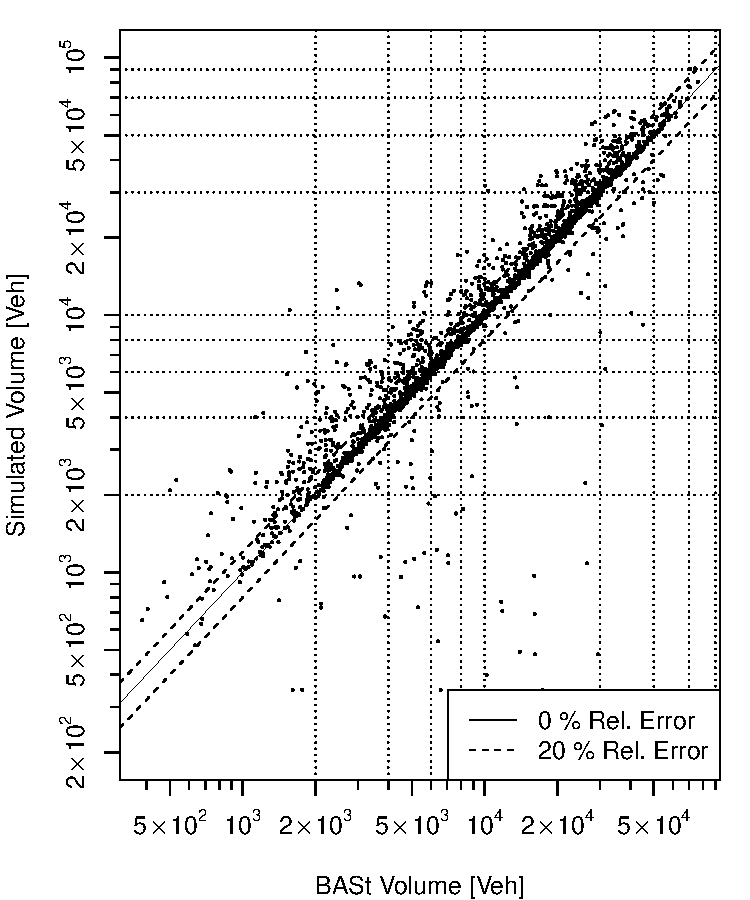
\includegraphics[width=0.45\textwidth, angle=0]{./scenarios/figures/germany-counts}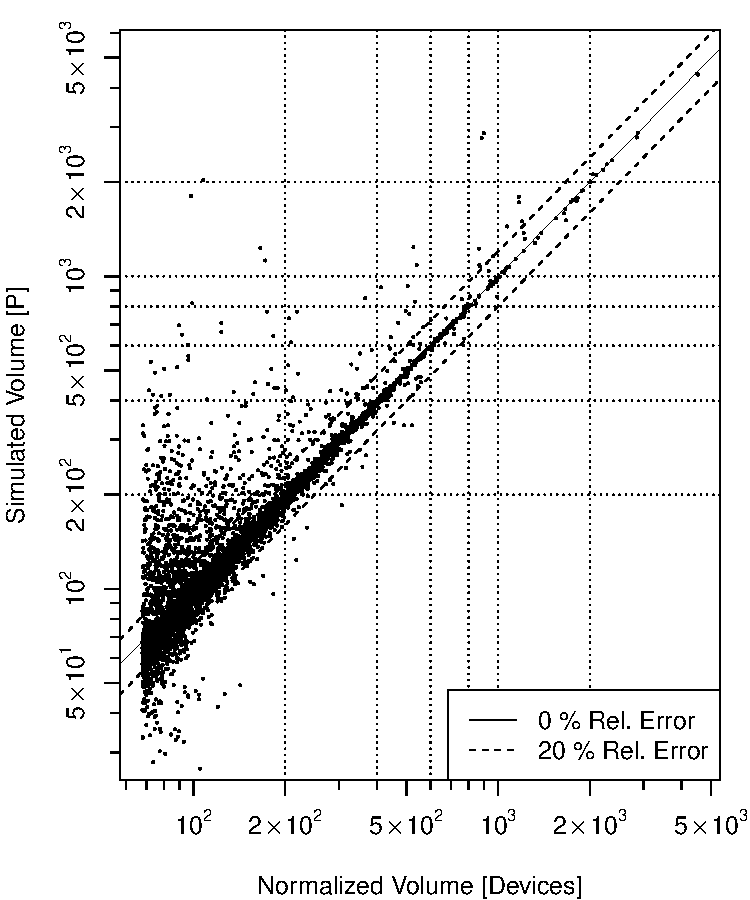
\includegraphics[width=0.45\textwidth, angle=0]{./scenarios/figures/germany-odcounts}}%
{}



